% Options for packages loaded elsewhere
\PassOptionsToPackage{unicode}{hyperref}
\PassOptionsToPackage{hyphens}{url}
\PassOptionsToPackage{dvipsnames,svgnames,x11names}{xcolor}
%
\documentclass[
  xelatex,
  ja=standard]{bxjsarticle}

\usepackage{amsmath,amssymb}
\usepackage{iftex}
\ifPDFTeX
  \usepackage[T1]{fontenc}
  \usepackage[utf8]{inputenc}
  \usepackage{textcomp} % provide euro and other symbols
\else % if luatex or xetex
  \usepackage{unicode-math}
  \defaultfontfeatures{Scale=MatchLowercase}
  \defaultfontfeatures[\rmfamily]{Ligatures=TeX,Scale=1}
\fi
\usepackage{lmodern}
\ifPDFTeX\else  
    % xetex/luatex font selection
  \setmainfont[BoldFont=Noto Sans CJK JP]{Noto Serif CJK JP}
\fi
% Use upquote if available, for straight quotes in verbatim environments
\IfFileExists{upquote.sty}{\usepackage{upquote}}{}
\IfFileExists{microtype.sty}{% use microtype if available
  \usepackage[]{microtype}
  \UseMicrotypeSet[protrusion]{basicmath} % disable protrusion for tt fonts
}{}
\makeatletter
\@ifundefined{KOMAClassName}{% if non-KOMA class
  \IfFileExists{parskip.sty}{%
    \usepackage{parskip}
  }{% else
    \setlength{\parindent}{0pt}
    \setlength{\parskip}{6pt plus 2pt minus 1pt}}
}{% if KOMA class
  \KOMAoptions{parskip=half}}
\makeatother
\usepackage{xcolor}
\setlength{\emergencystretch}{3em} % prevent overfull lines
\setcounter{secnumdepth}{5}
% Make \paragraph and \subparagraph free-standing
\ifx\paragraph\undefined\else
  \let\oldparagraph\paragraph
  \renewcommand{\paragraph}[1]{\oldparagraph{#1}\mbox{}}
\fi
\ifx\subparagraph\undefined\else
  \let\oldsubparagraph\subparagraph
  \renewcommand{\subparagraph}[1]{\oldsubparagraph{#1}\mbox{}}
\fi


\providecommand{\tightlist}{%
  \setlength{\itemsep}{0pt}\setlength{\parskip}{0pt}}\usepackage{longtable,booktabs,array}
\usepackage{calc} % for calculating minipage widths
% Correct order of tables after \paragraph or \subparagraph
\usepackage{etoolbox}
\makeatletter
\patchcmd\longtable{\par}{\if@noskipsec\mbox{}\fi\par}{}{}
\makeatother
% Allow footnotes in longtable head/foot
\IfFileExists{footnotehyper.sty}{\usepackage{footnotehyper}}{\usepackage{footnote}}
\makesavenoteenv{longtable}
\usepackage{graphicx}
\makeatletter
\def\maxwidth{\ifdim\Gin@nat@width>\linewidth\linewidth\else\Gin@nat@width\fi}
\def\maxheight{\ifdim\Gin@nat@height>\textheight\textheight\else\Gin@nat@height\fi}
\makeatother
% Scale images if necessary, so that they will not overflow the page
% margins by default, and it is still possible to overwrite the defaults
% using explicit options in \includegraphics[width, height, ...]{}
\setkeys{Gin}{width=\maxwidth,height=\maxheight,keepaspectratio}
% Set default figure placement to htbp
\makeatletter
\def\fps@figure{htbp}
\makeatother

\renewcommand{\thefootnote}{\arabic{footnote}}
\makeatletter
\@ifpackageloaded{tcolorbox}{}{\usepackage[skins,breakable]{tcolorbox}}
\@ifpackageloaded{fontawesome5}{}{\usepackage{fontawesome5}}
\definecolor{quarto-callout-color}{HTML}{909090}
\definecolor{quarto-callout-note-color}{HTML}{0758E5}
\definecolor{quarto-callout-important-color}{HTML}{CC1914}
\definecolor{quarto-callout-warning-color}{HTML}{EB9113}
\definecolor{quarto-callout-tip-color}{HTML}{00A047}
\definecolor{quarto-callout-caution-color}{HTML}{FC5300}
\definecolor{quarto-callout-color-frame}{HTML}{acacac}
\definecolor{quarto-callout-note-color-frame}{HTML}{4582ec}
\definecolor{quarto-callout-important-color-frame}{HTML}{d9534f}
\definecolor{quarto-callout-warning-color-frame}{HTML}{f0ad4e}
\definecolor{quarto-callout-tip-color-frame}{HTML}{02b875}
\definecolor{quarto-callout-caution-color-frame}{HTML}{fd7e14}
\makeatother
\makeatletter
\makeatother
\makeatletter
\makeatother
\makeatletter
\@ifpackageloaded{caption}{}{\usepackage{caption}}
\AtBeginDocument{%
\ifdefined\contentsname
  \renewcommand*\contentsname{目次}
\else
  \newcommand\contentsname{目次}
\fi
\ifdefined\listfigurename
  \renewcommand*\listfigurename{図一覧}
\else
  \newcommand\listfigurename{図一覧}
\fi
\ifdefined\listtablename
  \renewcommand*\listtablename{表一覧}
\else
  \newcommand\listtablename{表一覧}
\fi
\ifdefined\figurename
  \renewcommand*\figurename{図}
\else
  \newcommand\figurename{図}
\fi
\ifdefined\tablename
  \renewcommand*\tablename{表}
\else
  \newcommand\tablename{表}
\fi
}
\@ifpackageloaded{float}{}{\usepackage{float}}
\floatstyle{ruled}
\@ifundefined{c@chapter}{\newfloat{codelisting}{h}{lop}}{\newfloat{codelisting}{h}{lop}[chapter]}
\floatname{codelisting}{コード}
\newcommand*\listoflistings{\listof{codelisting}{コード一覧}}
\makeatother
\makeatletter
\@ifpackageloaded{caption}{}{\usepackage{caption}}
\@ifpackageloaded{subcaption}{}{\usepackage{subcaption}}
\makeatother
\makeatletter
\@ifpackageloaded{tcolorbox}{}{\usepackage[skins,breakable]{tcolorbox}}
\makeatother
\makeatletter
\@ifundefined{shadecolor}{\definecolor{shadecolor}{rgb}{.97, .97, .97}}
\makeatother
\makeatletter
\makeatother
\makeatletter
\makeatother
\ifLuaTeX
\usepackage[bidi=basic]{babel}
\else
\usepackage[bidi=default]{babel}
\fi
\babelprovide[main,import]{japanese}
% get rid of language-specific shorthands (see #6817):
\let\LanguageShortHands\languageshorthands
\def\languageshorthands#1{}
\ifLuaTeX
  \usepackage{selnolig}  % disable illegal ligatures
\fi
\usepackage[]{natbib}
\bibliographystyle{jecon}
\IfFileExists{bookmark.sty}{\usepackage{bookmark}}{\usepackage{hyperref}}
\IfFileExists{xurl.sty}{\usepackage{xurl}}{} % add URL line breaks if available
\urlstyle{same} % disable monospaced font for URLs
\hypersetup{
  pdftitle={デジタル化する社会},
  pdfauthor={土井翔平},
  pdflang={ja},
  colorlinks=true,
  linkcolor={NavyBlue},
  filecolor={Maroon},
  citecolor={NavyBlue},
  urlcolor={NavyBlue},
  pdfcreator={LaTeX via pandoc}}

\title{デジタル化する社会}
\usepackage{etoolbox}
\makeatletter
\providecommand{\subtitle}[1]{% add subtitle to \maketitle
  \apptocmd{\@title}{\par {\large #1 \par}}{}{}
}
\makeatother
\subtitle{技術政策学(データ科学編)}
\author{土井翔平}
\date{2023-05-15}

\begin{document}
\maketitle
\ifdefined\Shaded\renewenvironment{Shaded}{\begin{tcolorbox}[frame hidden, breakable, sharp corners, boxrule=0pt, interior hidden, borderline west={3pt}{0pt}{shadecolor}, enhanced]}{\end{tcolorbox}}\fi

\hypertarget{ux306fux3058ux3081ux306b}{%
\section*{はじめに}\label{ux306fux3058ux3081ux306b}}
\addcontentsline{toc}{section}{はじめに}

\begin{tcolorbox}[enhanced jigsaw, toptitle=1mm, colframe=quarto-callout-warning-color-frame, leftrule=.75mm, left=2mm, toprule=.15mm, colback=white, arc=.35mm, bottomrule=.15mm, titlerule=0mm, bottomtitle=1mm, coltitle=black, title=\textcolor{quarto-callout-warning-color}{\faExclamationTriangle}\hspace{0.5em}{警告}, breakable, rightrule=.15mm, opacityback=0, opacitybacktitle=0.6, colbacktitle=quarto-callout-warning-color!10!white]

日進月歩の分野なので、本章の内容はすぐに古いものになる(or既にそうであるかもしれない)点に注意。

\end{tcolorbox}

\textbf{人工知能} (artificial intelligence) とは?

\begin{itemize}
\tightlist
\item
  コンピュータ(機械)が人間のように意思をもって、自律的に認識・判断・行動する?
\end{itemize}

\(\leadsto\)機械学習について学ぶことで(昨今、話題になっている)人工知能について理解する。

なぜ\textbf{機械学習} (machine learning) か?

\begin{figure}[htpb]

{\centering 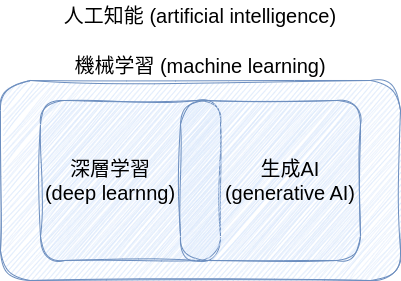
\includegraphics[width=0.8\textwidth,height=\textheight]{figures/ml_ai.drawio.png}

}

\caption{人工知能、機械学習、深層学習、生成AIの関係}

\end{figure}

機械学習:データから一定のパターンを機械(パソコン)が学習し、\textbf{予測をする}。

近年の人工知能\(\approx\)機械学習のブレイクスルー

\begin{enumerate}
\def\labelenumi{\arabic{enumi}.}
\tightlist
\item
  ビッグデータの利活用
\item
  深層学習(およびその発展形)の発明
\item
  豊富な計算資源
\end{enumerate}

\(\leadsto\)特に(我々にとって)重要な1点目と2点目に焦点

\hypertarget{ux30d3ux30c3ux30b0ux30c7ux30fcux30bf}{%
\section{ビッグデータ}\label{ux30d3ux30c3ux30b0ux30c7ux30fcux30bf}}

インターネット空間の拡大やセンシング技術の向上(スマートフォン、衛星写真)により、\textbf{ビッグデータ}を収集することができる。

\begin{itemize}
\tightlist
\item
  \textbf{ビッグデータ}:人間の様々な活動が粒度の高い(従って大規模な)データとして記録される。
\item
  インターネットはそのようなデータを生み出す最初の空間だったが、最近ではインターネットに限られない。
\end{itemize}

\(\leadsto\)ビッグデータの特徴は大規模であること自体ではなく、\textbf{粒度}
(granularity) が高い(データが細かい)ことである。

\begin{enumerate}
\def\labelenumi{\arabic{enumi}.}
\tightlist
\item
  多様性 (variery) :国レベルではなく地方自治体、個人レベル

  \begin{itemize}
  \tightlist
  \item
    小さいレベルのデータから全体を作ることはできるが、その逆ではない。
  \end{itemize}
\item
  速度 (velocity) :年単位ではなく月単位、分単位

  \begin{itemize}
  \tightlist
  \item
    一定の間隔や一時的なデータ収集ではなく、always-onが理想である。
  \end{itemize}
\item
  量 (volume) :多様性と速度の結果としての大規模データ
\end{enumerate}

\(\leadsto\)ビッグデータを解析できる機械学習(特に深層学習)の登場により、ビッグデータの価値が生まれ始めている。

\hypertarget{ux30d3ux30c3ux30b0ux3067ux306fux306aux3044ux30c7ux30fcux30bf}{%
\subsection{ビッグではないデータ}\label{ux30d3ux30c3ux30b0ux3067ux306fux306aux3044ux30c7ux30fcux30bf}}

伝統的なデータは分析レベルが荒いデータである。

\begin{itemize}
\tightlist
\item
  \href{https://ucdp.uu.se/encyclopedia}{UCDPの紛争データ}
\item
  \href{https://www.v-dem.net/}{V-Demの政治体制データ}
\item
  \href{http://www.masaki.j.u-tokyo.ac.jp/utas/utasindex.html}{東大・朝日の世論調査}
\end{itemize}

多くの場合、

\begin{itemize}
\tightlist
\item
  国レベルに集計したり、一部の個人のみを対象
\item
  毎年、イベントごとなど特定の時点のみを対象
\end{itemize}

としている。

\hypertarget{ux5730ux7406ux60c5ux5831ux30b7ux30b9ux30c6ux30e0}{%
\subsection{地理情報システム}\label{ux5730ux7406ux60c5ux5831ux30b7ux30b9ux30c6ux30e0}}

GPS付きスマートフォンのデータにより個人の位置情報がほぼリアルタイムで計測できる。

\begin{itemize}
\tightlist
\item
  外出者の数や移動経路が分かり、感染症対策に利活用できる。
\end{itemize}

\textbf{地理情報システム} (geospatial information system: GIS)
の発展・普及によって地理空間データの利活用が進んでいる。

人工衛星の写真から経済発展や森林破壊の度合いを測定することができる。

\(\leadsto\)リモート・センシングによりこれまでアクセスできなかったデータを取得できる。

\begin{itemize}
\tightlist
\item
  統計が怪しい、取ることのできない地域のデータ
\item
  行政単位よりも細かい地域区分でデータ
\end{itemize}

\begin{figure}

\begin{minipage}[t]{0.50\linewidth}

{\centering 

\raisebox{-\height}{

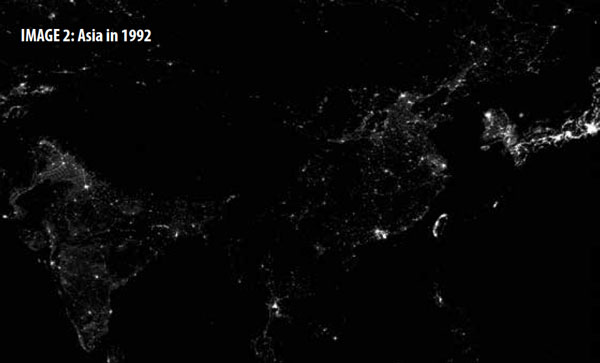
\includegraphics{figures/nightlight1.jpg}

}

}

\end{minipage}%
%
\begin{minipage}[t]{0.50\linewidth}

{\centering 

\raisebox{-\height}{

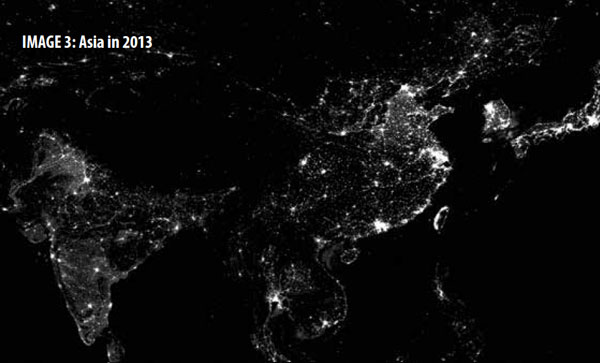
\includegraphics{figures/nightlight2.jpg}

}

}

\end{minipage}%
\newline
\begin{minipage}[t]{0.50\linewidth}

{\centering 

\href{https://www.imf.org/en/Publications/fandd/issues/2019/09/satellite-images-at-night-and-economic-growth-yao}{Satellite
images of the earth at night reveal the pace of economic growth and much
more}

}

\end{minipage}%

\end{figure}

通話履歴から個人の(従って地域の)豊かさを予測することができる。

\begin{itemize}
\tightlist
\item
  \href{https://ict4d.jp/2017/07/01/mobile-poverty/}{ルワンダ}最大の携帯電話会社の協力を得て分析を行った。
\end{itemize}

\begin{figure}[htpb]

{\centering \includegraphics{big_data_files/mediabag/350_1073_f2.jpeg}

}

\caption{\citet{blumenstock2015}}

\end{figure}

街中にある監視カメラと画像認識技術を組み合わせることで、犯人の迅速な逮捕や犯罪防止に役立っている。

\begin{itemize}
\tightlist
\item
  プライバシーの侵害の懸念はある。
\item
  中国は\href{https://www.nikkei.com/article/DGXMZO53393500W9A211C1000000/}{監視技術を外国に輸出}している。
\end{itemize}

GISを(無料で)使えるサービスがある。

\begin{itemize}
\tightlist
\item
  \href{https://resas.go.jp/}{RESAS}
\item
  \href{https://jstatmap.e-stat.go.jp/trialstart.html}{jSTAT MAP}
\item
  \href{https://qgis.org/ja/site/forusers/download.html}{QGIS}
\end{itemize}

\hypertarget{ux4f01ux696dux30c7ux30fcux30bf}{%
\subsection{企業データ}\label{ux4f01ux696dux30c7ux30fcux30bf}}

株式保有のデータを用いて、株式ネットワークのデータを構築することができる。

\(\leadsto\)直接的だけでなく間接的に、どのような株主が、どのような企業を、どの程度接続しているのかが分かる。

\begin{figure}[htpb]

{\centering 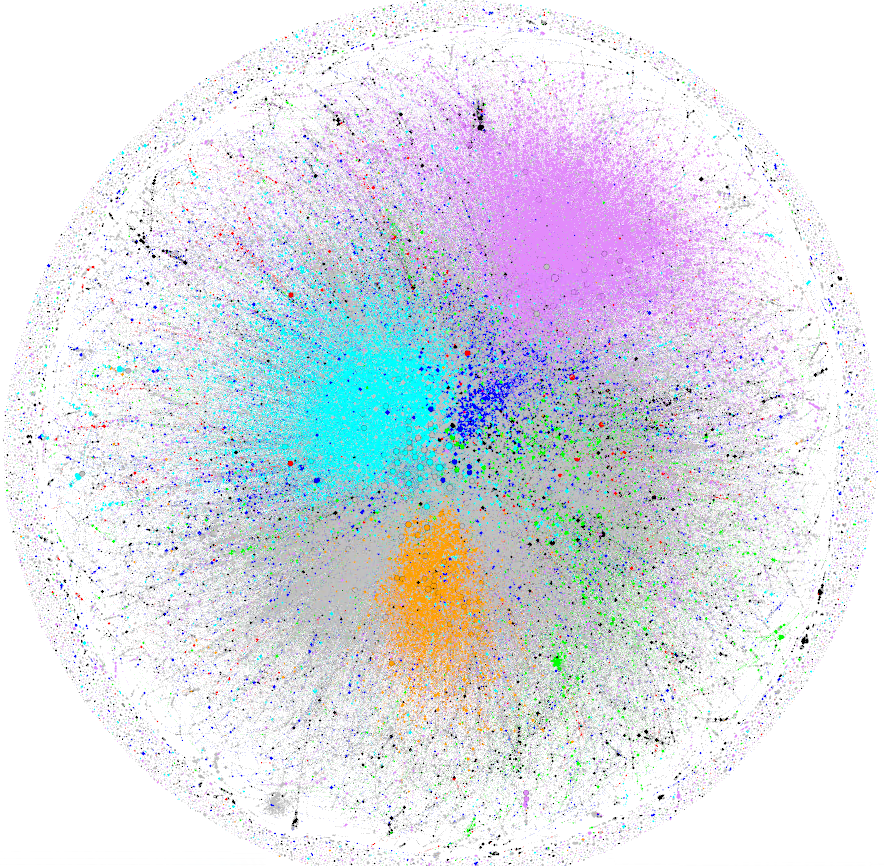
\includegraphics[width=0.5\textwidth,height=\textheight]{figures/ownership.png}

}

\caption{2020年のグローバルな株式ネットワーク}

\end{figure}

\begin{itemize}
\tightlist
\item
  間接的支配を含めると、中国政府は世界最大の株主である。
\item
  一般的に販売されている金融商品の約9割が軍事企業や環境破壊企業に繋がっている。
\item
  \href{https://business.nikkei.com/atcl/gen/19/00351/110900058/}{「隠れ株主」を探せ:米テスラ、サプライチェーンの「身体検査」}
\end{itemize}

\hypertarget{ux30c7ux30b8ux30bfux30ebux30d2ux30e5ux30fcux30deux30cbux30c6ux30a3ux30fcux30ba}{%
\subsection{デジタル・ヒューマニティーズ}\label{ux30c7ux30b8ux30bfux30ebux30d2ux30e5ux30fcux30deux30cbux30c6ux30a3ux30fcux30ba}}

人文学(特に歴史学)にデジタル技術を取り入れている分野を\textbf{デジタル・ヒューマニティ}
(digital humanity) と呼ぶ。

電子書籍によって大量の書籍を電子的に処理することが可能になった。

\begin{itemize}
\tightlist
\item
  \href{https://books.google.com/ngrams}{Google Ngram
  Viewer}や\href{https://lab.ndl.go.jp/service/ngramviewer/}{NDL Ngram
  Viewer}によって1800年ごろから書籍における単語の頻度を見ることができる。
\end{itemize}

画像認識の技術を応用して\href{http://codh.rois.ac.jp/project/index.html.ja}{日本史の資料のデジタル化}が進んでいる。

\begin{itemize}
\tightlist
\item
  \href{http://codh.rois.ac.jp/kuronet/}{くずし字OCR}
\item
  \href{http://codh.rois.ac.jp/edo-cooking/}{江戸料理レシピ}
\item
  \href{http://codh.rois.ac.jp/ukiyo-e/index.html.ja}{浮世絵顔データ}
\end{itemize}

\hypertarget{ux30a4ux30f3ux30bfux30fcux30cdux30c3ux30c8ux7a7aux9593}{%
\section{インターネット空間}\label{ux30a4ux30f3ux30bfux30fcux30cdux30c3ux30c8ux7a7aux9593}}

21世紀の特徴の1つはインターネット空間の登場と拡大である。

\(\leadsto\)情報通信コストが限りなく下がり、経済活動だけでなく言論空間もオンライン上に構築された。

\begin{figure}[htpb]

{\centering \includegraphics{big_data_files/mediabag/hilbert_worlds_2011_.png}

}

\caption{\citet{salganik2019}}

\end{figure}

ビッグデータという観点からすると、膨大な量のデータが日々、作られている。

\begin{itemize}
\tightlist
\item
  \textbf{テキスト}データ
\item
  \textbf{画像}データ
\item
  音声データ
\item
  映像データ
\end{itemize}

\(\leadsto\)人工知能の誕生によって、はじめてビッグデータに価値が生まれ、インターネット空間が(さらに)変容しつつある。

なぜGoogleは強いのか?

\begin{itemize}
\tightlist
\item
  Google Flu
  Trendsというインフルエンザに関する検索傾向からインフルエンザの感染を予測するサービスがあった(現在は中止)。
\end{itemize}

\begin{figure}[htpb]

{\centering \includegraphics{big_data_files/mediabag/keithgraph-768x446.jpeg}

}

\caption{\href{https://www.wbur.org/news/2013/01/13/google-flu-trends-cdc}{Is
`Google Flu Trends' Prescient Or Wrong?}}

\end{figure}

\begin{itemize}
\tightlist
\item
  \href{https://trends.google.co.jp/trends/}{Googleトレンド}で検索傾向を調べることができる。
\end{itemize}

しかも、人々が\textbf{アノテーション}(情報の付加)をしてくれている。

\begin{itemize}
\tightlist
\item
  商品やお店のレビュー
\item
  画像のタグ付け(画像つきツイート)、地理情報
\end{itemize}

\hypertarget{ux30bdux30fcux30b7ux30e3ux30ebux30cdux30c3ux30c8ux30efux30fcux30af}{%
\subsection{ソーシャル・ネットワーク}\label{ux30bdux30fcux30b7ux30e3ux30ebux30cdux30c3ux30c8ux30efux30fcux30af}}

\textbf{デジタル・フットプリント}(インターネット上の行動履歴)から個人的属性を予測できる。

\(\leadsto\)個人に焦点を当てた(\textbf{パーソナライズ}した)マーケティングを行える。

\begin{itemize}
\tightlist
\item
  インターネットの広告、eコマースにおける推薦
\end{itemize}

\(\leadsto\)ユーザーは自由に情報を検索して、選択しているつもりでも、表示される情報は誘導されている。

Netflixはデータを公開して予測コンペ (Netflix Prize) を行っていた。

公開されたデータは匿名であるが、視聴履歴から個人を特定することができることが分かる。

\begin{itemize}
\tightlist
\item
  脱匿名化、再識別などと呼ぶ。
\end{itemize}

\(\leadsto\)政治信条や性的志向が判明する危険性がある。

SNSは豊富な情報を持つビッグデータである。

\begin{itemize}
\tightlist
\item
  個人レベル
\item
  always-on
\item
  テキスト、画像と繋がり(ネットワーク)
\end{itemize}

\(\leadsto\)政治信条や性的志向が暴露されてしまう危険性がある。

\begin{itemize}
\tightlist
\item
  \href{https://www.axion.zone/private-traits-and-attributes-are-predictable-from-digital-records-of-human-behavior/}{とある研究}ではFacebookの「いいね
  (like) 」を使って個人属性を予測した。
\end{itemize}

\begin{figure}[htpb]

{\centering \includegraphics{big_data_files/mediabag/pnas.1218772110fig02.jpeg}

}

\caption{\citet{kosinski2013}}

\end{figure}

\begin{itemize}
\tightlist
\item
  ケンブリッジ・アナリティカ社がFacebook上で選挙介入を行ったと指摘されている。
\end{itemize}

\hypertarget{snsux4e0aux306eux30b3ux30dfux30e5ux30cbux30c6ux30a3}{%
\subsection{SNS上のコミュニティ}\label{snsux4e0aux306eux30b3ux30dfux30e5ux30cbux30c6ux30a3}}

人々は同じ意見を持っている人同士で繋がる傾向を\textbf{ホモフィリー}と呼ぶ。

\begin{itemize}
\tightlist
\item
  トランプのフォロワーはクリントンのフォロワーと繋がりにくい。
\end{itemize}

\begin{figure}[htpb]

{\centering 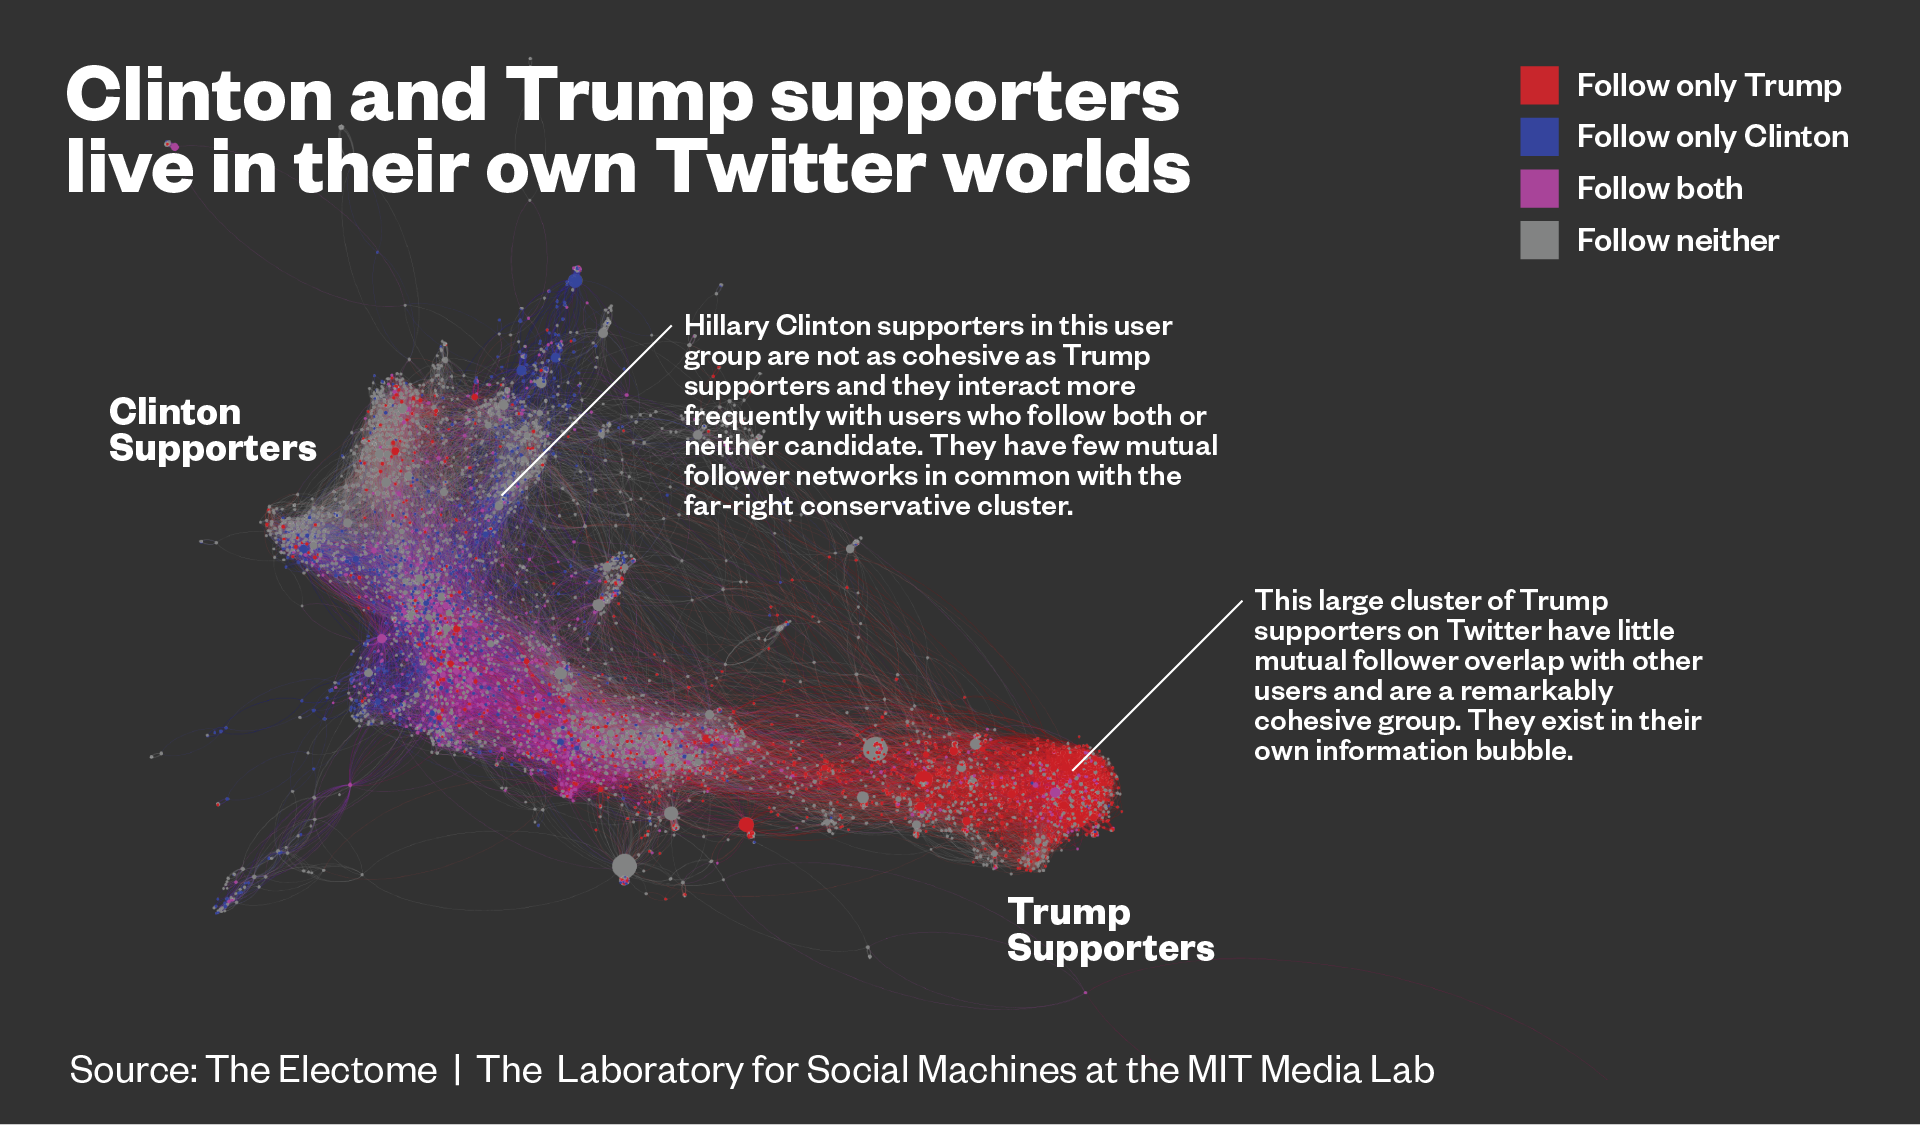
\includegraphics{figures/twitter1.png}

}

\caption{\href{https://www.vice.com/en/article/d3xamx/journalists-and-trump-voters-live-in-separate-online-bubbles-mit-analysis-shows}{Journalists
and Trump voters live in separate online bubbles, MIT analysis shows}}

\end{figure}

同質的なコミュニティで意見が反射、増幅して信念が強化される\textbf{エコー・チェンバー}が生じる。

\begin{itemize}
\tightlist
\item
  人種差別についてリベラルでしか議論されない。
\item
  移民や銃については両方で議論されているが、繋がってはいない。
\end{itemize}

\begin{figure}[htpb]

{\centering 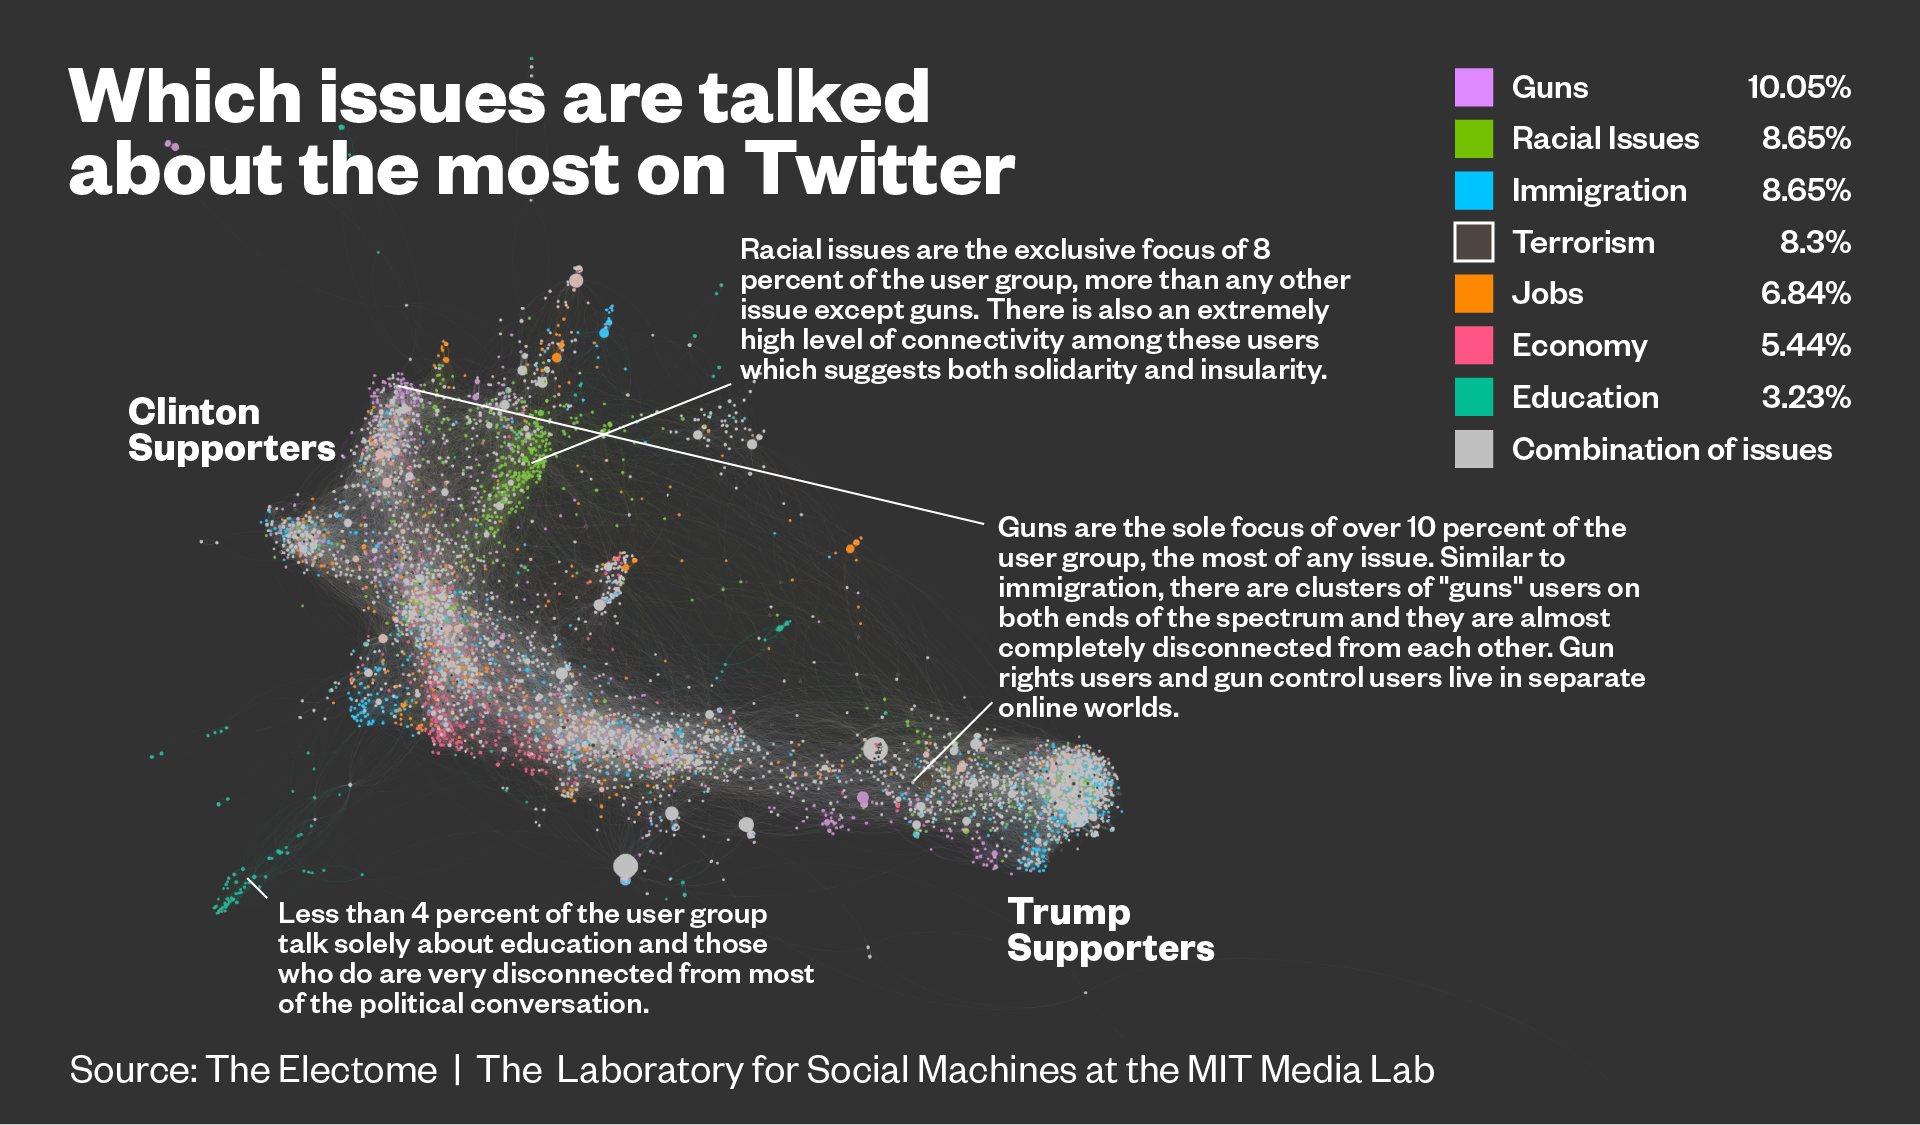
\includegraphics{figures/twitter2.png}

}

\caption{\href{https://www.vice.com/en/article/d3xamx/journalists-and-trump-voters-live-in-separate-online-bubbles-mit-analysis-shows}{Journalists
and Trump voters live in separate online bubbles, MIT analysis shows}}

\end{figure}

SNSがパーソナライズされる(フォローの推薦)ことで投稿内容やユーザーが限定される。

\(\leadsto\)(本人の意図によらず)見たくない情報がSNS上から除去される\textbf{フィルター・バブル}ができる。

\begin{figure}[htpb]

{\centering 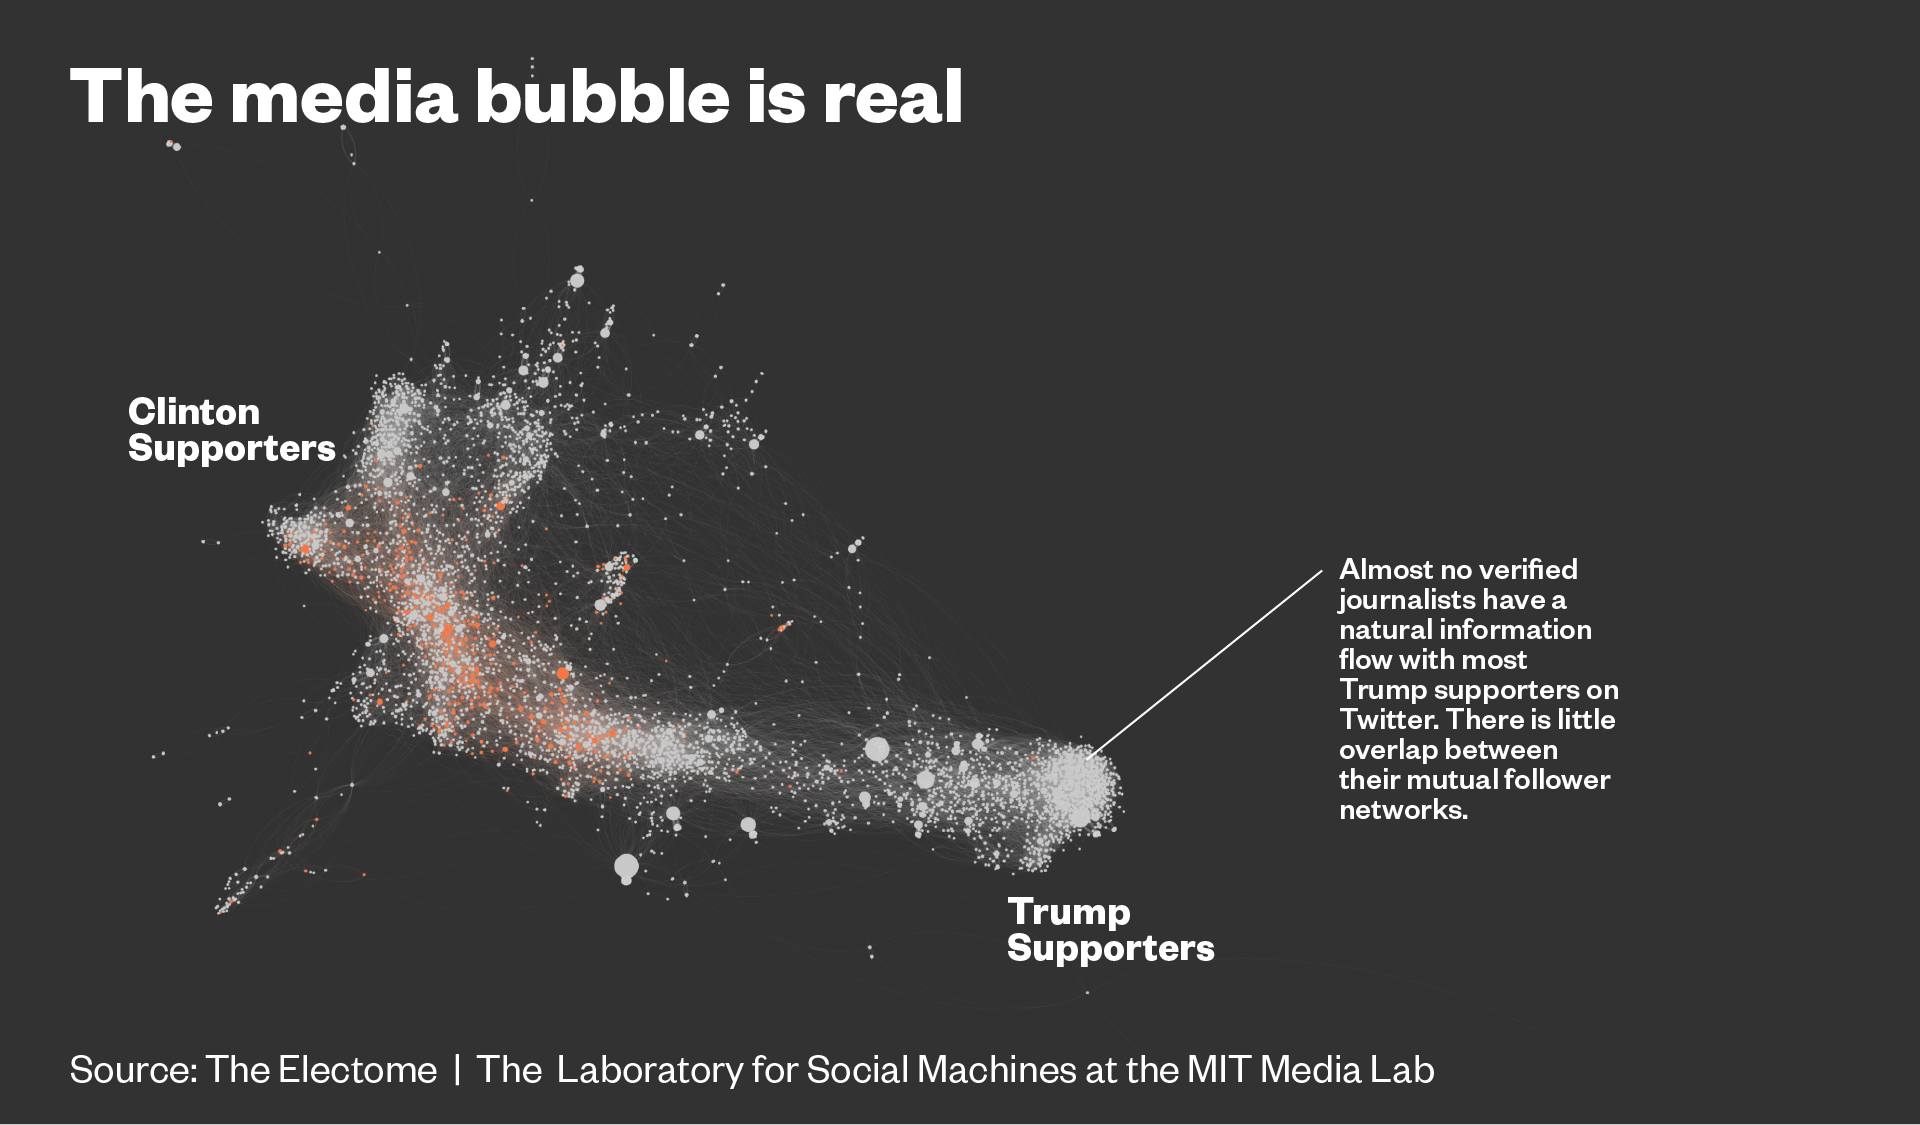
\includegraphics{figures/twitter3.png}

}

\caption{\href{https://www.vice.com/en/article/d3xamx/journalists-and-trump-voters-live-in-separate-online-bubbles-mit-analysis-shows}{Journalists
and Trump voters live in separate online bubbles, MIT analysis shows}}

\end{figure}

ホモフィリーが正しいのだとすれば、SNS上の繋がりから政治的イデオロギーも分かる。

\begin{itemize}
\tightlist
\item
  SNS上を通じて世論や分極化をリアルタイムに観測できる。
\item
  SNS上の情報で個人の政治的傾向が分かってしまう。
\end{itemize}

\begin{figure}[htpb]

{\centering \includegraphics{big_data_files/mediabag/5-Figure1-1.png}

}

\caption{\citet{barbera2015}}

\end{figure}

\hypertarget{snsux3068ux5206ux6975ux5316ux5206ux65ad}{%
\subsection{SNSと分極化・分断}\label{snsux3068ux5206ux6975ux5316ux5206ux65ad}}

分極化
(polarization):社会において意見(特にイデオロギー)が分断し、それぞれ極端になっていく現象

\(\leadsto\)インターネットは分極化を加速させるのか?

\citet[第5章]{inamasu2022}によれば、そこまでの影響力は大きくない。

\begin{itemize}
\tightlist
\item
  アルゴリズムによる表示 (exposed) よりも、自身の選択 (selected)
  の方が異なるイデオロギーの記事にアクセスしにくい(あるいは大差はない)。
\end{itemize}

\begin{figure}[htpb]

{\centering 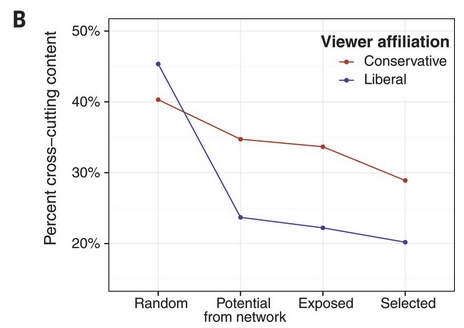
\includegraphics{figures/bakshy.png}

}

\caption{bakshy2015}

\end{figure}

\begin{itemize}
\tightlist
\item
  ニュースアグリゲーターよりもSNSなどのほうが多様な意見のサイトにアクセスしやすい。
\end{itemize}

\begin{figure}[htpb]

{\centering 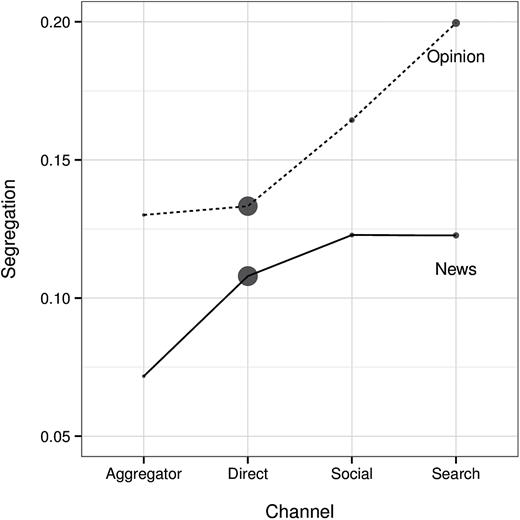
\includegraphics{figures/flaxman1.jpeg}

}

\caption{\citet{flaxman2016}}

\end{figure}

\begin{itemize}
\tightlist
\item
  ニュースアグリゲーターやSNSは異なる意見のサイトにアクセスしやすい。
\end{itemize}

\begin{figure}[htpb]

{\centering 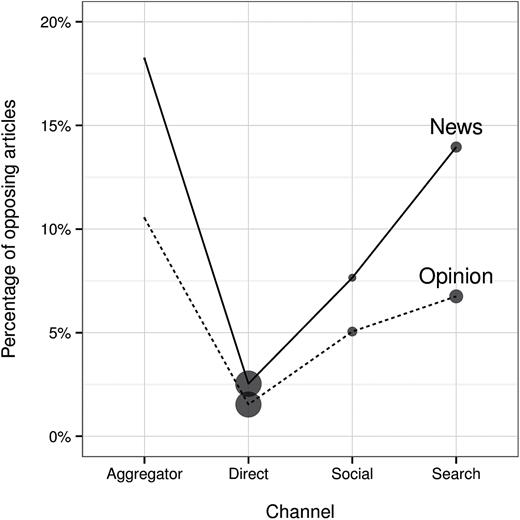
\includegraphics{figures/flaxman2.jpeg}

}

\caption{\citet{flaxman2016}}

\end{figure}

\(\leadsto\)アルゴリズムによる分断よりも、自らの選択?

\hypertarget{ux4e2dux56fdux306bux3088ux308bsnsux691cux95b2}{%
\subsection{中国によるSNS検閲}\label{ux4e2dux56fdux306bux3088ux308bsnsux691cux95b2}}

中国ではTwitterなどは利用できないが、類似のサービスが利用されているが、検閲されているかもしれない。

\(\leadsto\)\href{https://ipsj.ixsq.nii.ac.jp/ej/?action=pages_view_main\&active_action=repository_view_main_item_detail\&item_id=199708\&item_no=1\&page_id=13\&block_id=8}{とある研究}によって、情報を隠すという検閲により、隠したい中国政府の意図が分かってしまった。

どうやって検閲を見つけるのか?

\begin{enumerate}
\def\labelenumi{\arabic{enumi}.}
\tightlist
\item
  人力検閲で削除される前に\textbf{スクレイピング}する。
\item
  実際に中国のSNSアカウントを作り、投稿する。
\item
  実際に中国のSNSサービスを作り、マニュアルを見る。
\end{enumerate}

自動検閲される確率は(2013年時点では)ほとんどない。

\begin{figure}[htpb]

{\centering 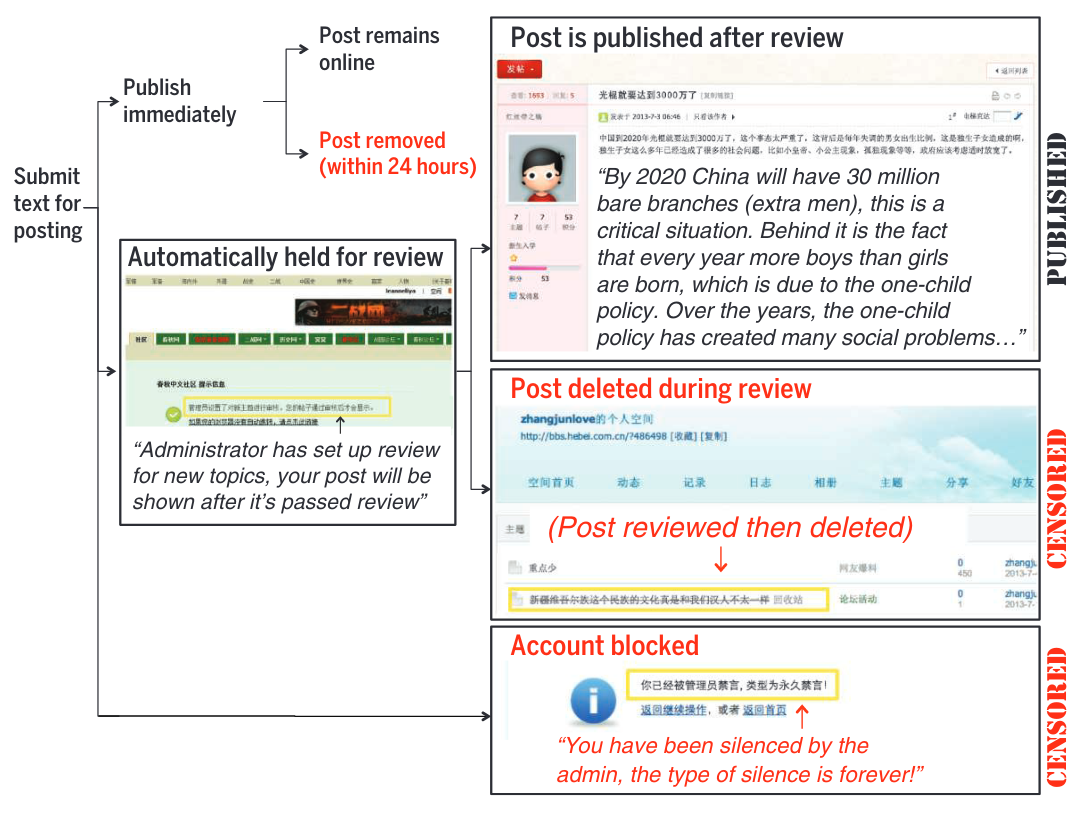
\includegraphics{figures/censorship1.png}

}

\caption{\citet{king2014}}

\end{figure}

中国で検閲されやすい内容は

\begin{enumerate}
\def\labelenumi{\arabic{enumi}.}
\tightlist
\item
  デモや集会に繋がる行動
\item
  検閲の批判
\item
  ポルノグラフィー
\end{enumerate}

に関するものである。

\begin{figure}[htpb]

{\centering 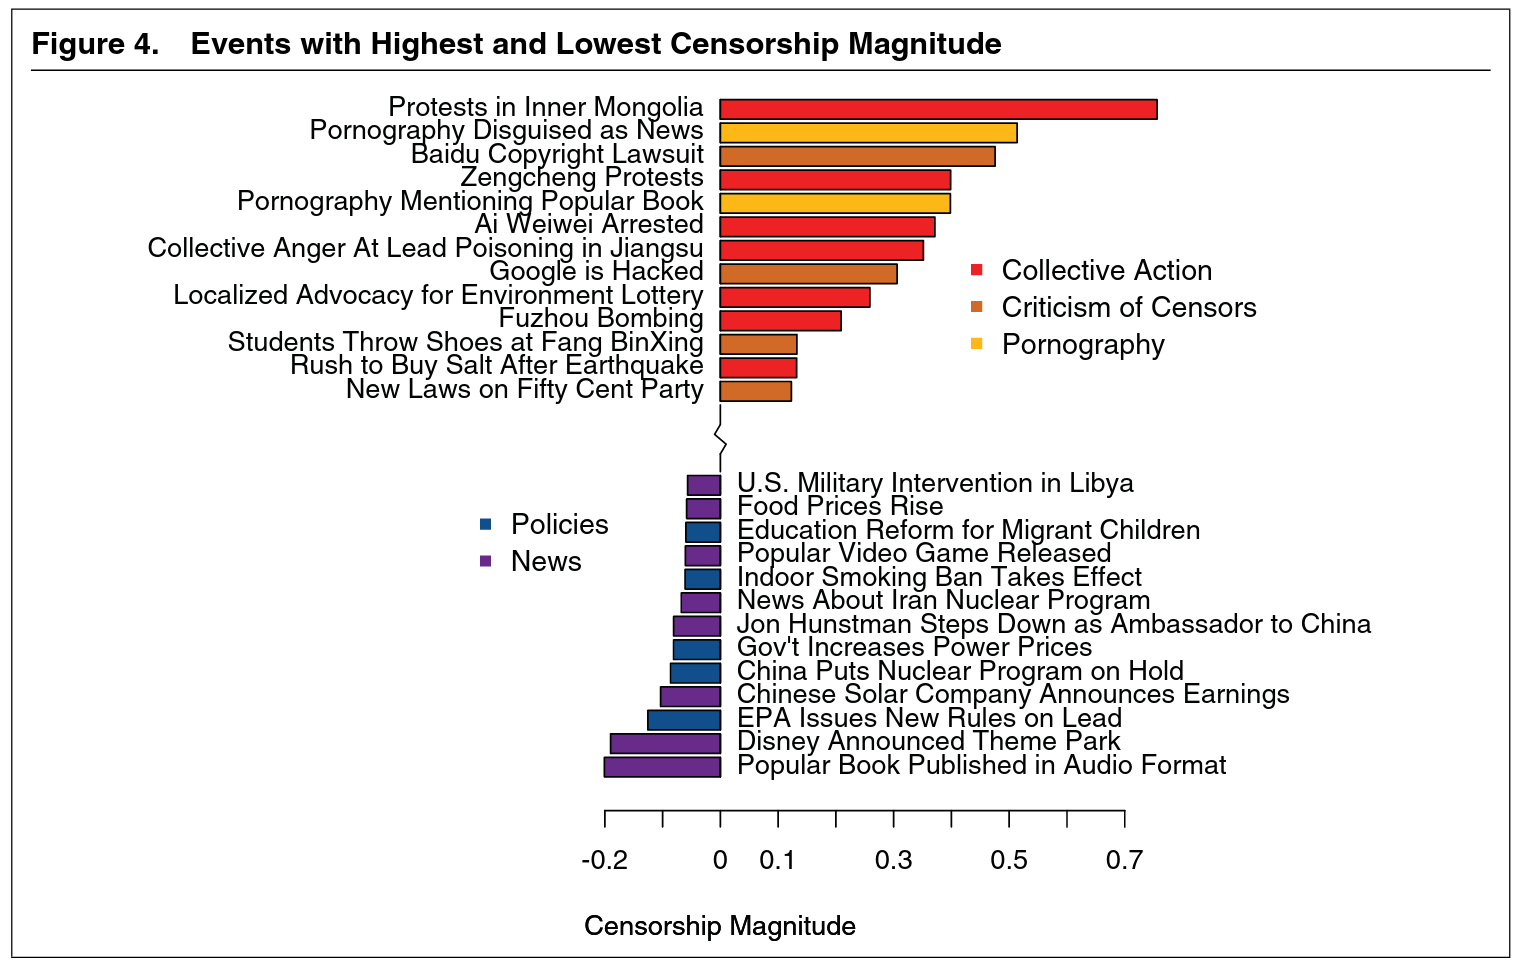
\includegraphics{figures/censorship2.png}

}

\caption{\citet{king2013}}

\end{figure}

検閲される確率は政府に対して肯定的であるか批判的であるかは「関係がない」。

\begin{itemize}
\tightlist
\item
  天安門事件に関する投稿だからといって削除されるとは限らない。
\end{itemize}

\begin{figure}[htpb]

{\centering 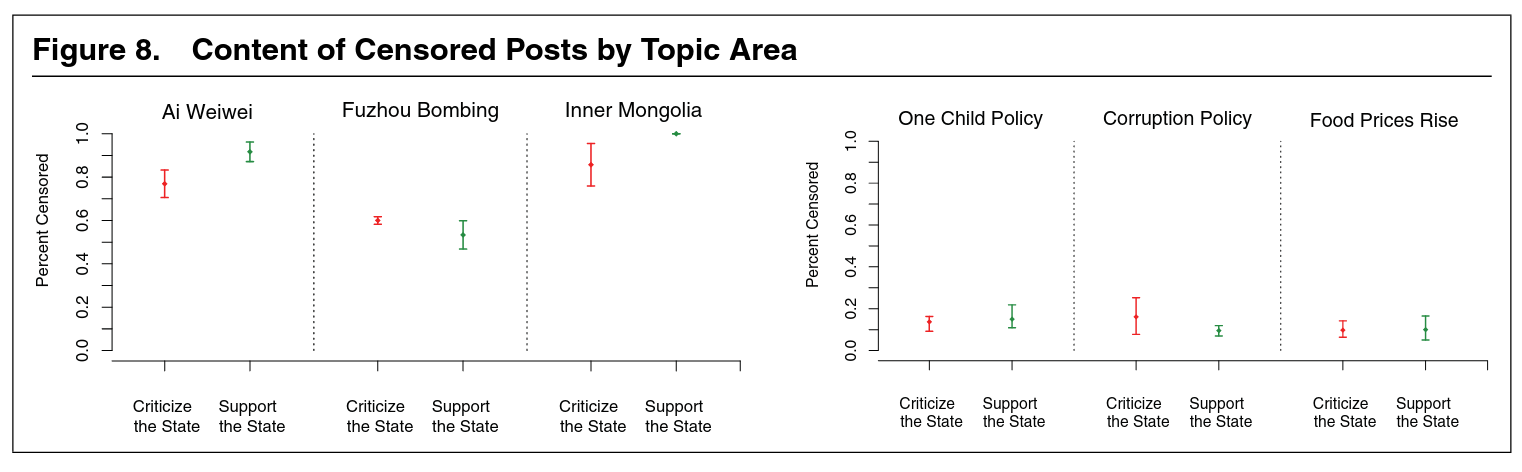
\includegraphics{figures/censorship3.png}

}

\caption{\citet{king2013}}

\end{figure}

中国のSNSでは五毛党 (50 Cent Party) が世論誘導 (astroturfing)
を行っていると考えられている。

\begin{itemize}
\tightlist
\item
  とある地区の五毛党のリストがリークした。
\end{itemize}

\(\leadsto\)機械学習によって五毛党のアカウントを予測し、それらの投稿の内容も分類できる。

五毛党は協調して投稿している。

五毛党は外国の批判や論争への参加は\textbf{していない}。

\begin{itemize}
\tightlist
\item
  愛国心を煽る表現
\item
  政府の政策の紹介
\item
  論争的ではない政府の称賛
\end{itemize}

\(\leadsto\)政府の意見を広めるというより、不都合な情報から目を逸らそうとしているのでは?

\begin{figure}[htpb]

{\centering 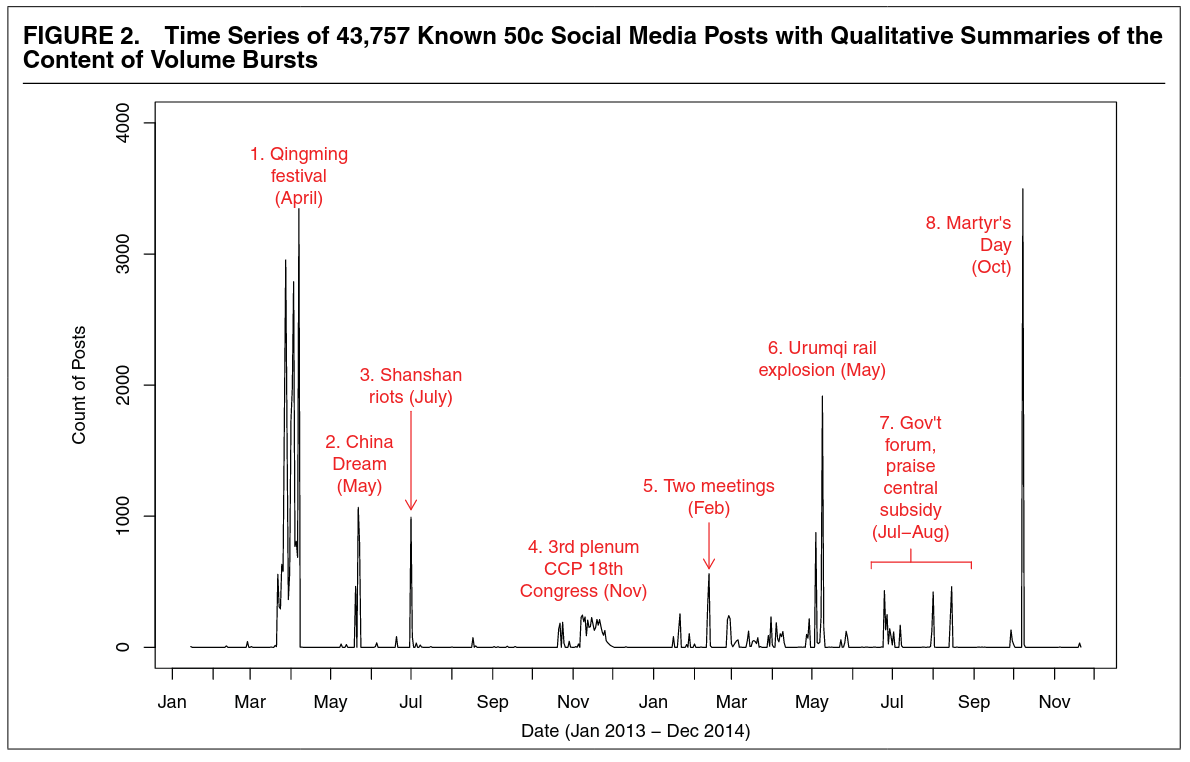
\includegraphics{figures/censorship4.png}

}

\caption{\citet{king2017}}

\end{figure}

\begin{figure}[htpb]

{\centering 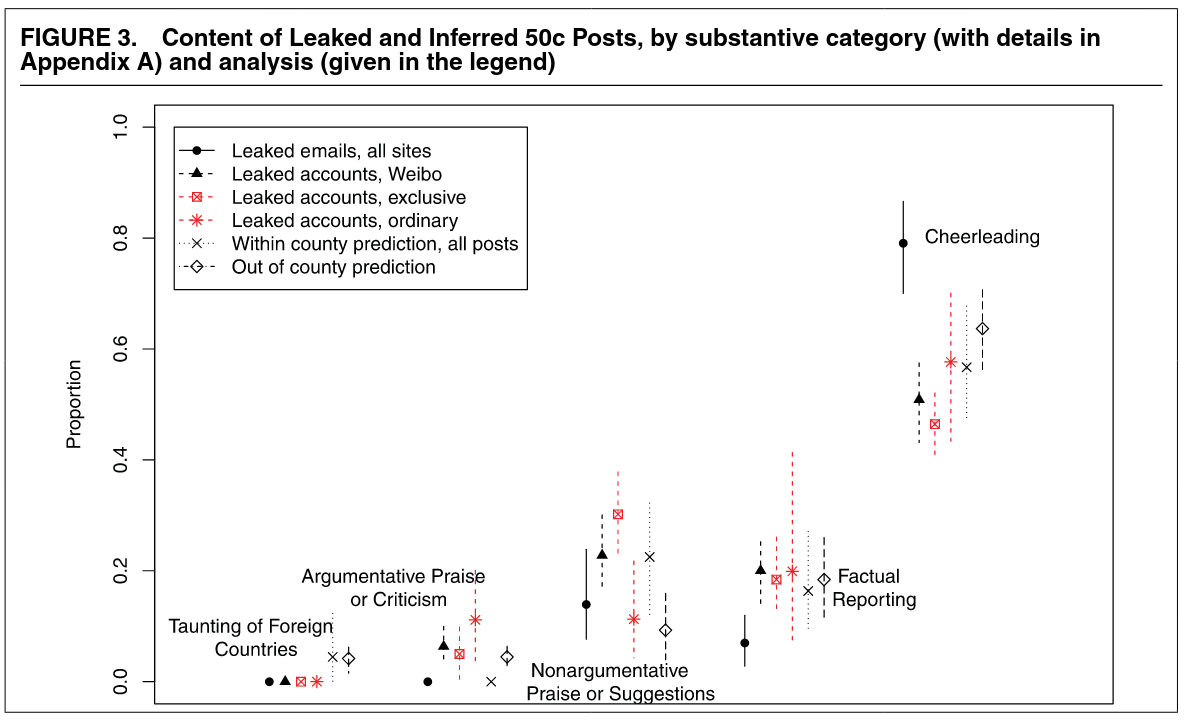
\includegraphics{figures/censorship5.png}

}

\caption{\citet{king2017}}

\end{figure}

\hypertarget{ux30aaux30f3ux30e9ux30a4ux30f3ux5b9fux9a13}{%
\subsection{オンライン実験}\label{ux30aaux30f3ux30e9ux30a4ux30f3ux5b9fux9a13}}

\textbf{A/Bテスト}とはランダムに異なるウェブサイトを表示し、収益の高いウェブサイトを見つける実験のことである。\footnote{実験については統計的因果推論において解説する。}

\begin{itemize}
\tightlist
\item
  オバマ元大統領は選挙資金の寄付を受け付けるサイトのデザインでA/Bテストを行い、約6000万ドルの寄付増加に繋がったと言われている。
\end{itemize}

\begin{figure}[htpb]

{\centering \includegraphics{big_data_files/mediabag/82330bae6a74b04d0087.png}

}

\caption{\href{https://juicer.cc/articles/archives/1273/}{あの大統領も140\%の成果改善。アメリカ大統領とA/Bテストの意外な関係}}

\end{figure}

オンライン上では(しばしば利用者が知らないうちに)実験が行われている。

\begin{itemize}
\tightlist
\item
  Facebookの\href{https://www.afpbb.com/articles/-/2900894}{選挙実験}では友人が投票に行ったことを知ると、投票率が上がることが分かった。
\end{itemize}

\begin{figure}[htpb]

{\centering \includegraphics{big_data_files/mediabag/41586_2012_Article_B.jpg}

}

\caption{\citet{bond2012}}

\end{figure}

\begin{itemize}
\tightlist
\item
  Facebookの\href{https://www.itmedia.co.jp/news/articles/1406/29/news007.html}{感情実験}ではTL上にネガティブな投稿が表示されなくなると、ポジティブな投稿が増える(その逆も然り)ことが分かった。
\end{itemize}

\begin{figure}[htpb]

{\centering \includegraphics{big_data_files/mediabag/yu_emotion.jpg}

}

\caption{\citet{kramer2014}}

\end{figure}

\hypertarget{ux5f71ux97ffux5de5ux4f5c}{%
\subsection{影響工作}\label{ux5f71ux97ffux5de5ux4f5c}}

影響工作 (influence
operation):フェイクニュースなどを通じて世論に影響を与えようとする行動

\(\leadsto\)インターネット空間ではボットによる情報提供が容易に\citep{lazer2009, ferrara2016}。

\begin{itemize}
\tightlist
\item
  2016年のアメリカ大統領選ではトランプ支持のツイートを(特に接戦州で)ボットが共有
\item
  イギリスのEU離脱投票の際にも賛成派と反対派のボットが情報を拡散
\end{itemize}

信頼のできないボット(赤い点)が特定のユーザーをリツイートしている。

\begin{figure}[htpb]

{\centering \includegraphics{big_data_files/mediabag/42001_2021_139_Fig1_.png}

}

\caption{\citet{xu2022}}

\end{figure}

\begin{itemize}
\tightlist
\item
  信頼のできないボットは陰謀論者をリツイート
\item
  スーパスプレッダーとなるボット
\end{itemize}

\href{https://www.natureasia.com/ja-jp/ndigest/v15/n5/\%E3\%83\%95\%E3\%82\%A7\%E3\%82\%A4\%E3\%82\%AF\%E3\%83\%8B\%E3\%83\%A5\%E3\%83\%BC\%E3\%82\%B9\%E3\%81\%AF\%E9\%80\%9F\%E3\%81\%8F\%E5\%BA\%83\%E3\%81\%8F\%E4\%BC\%9D\%E3\%82\%8F\%E3\%82\%8B/92004}{とある研究}によれば、フェイクニュースは正しいニュースよりもリツイートされやすく、早く、広く拡散する。

\begin{figure}[htpb]

{\centering 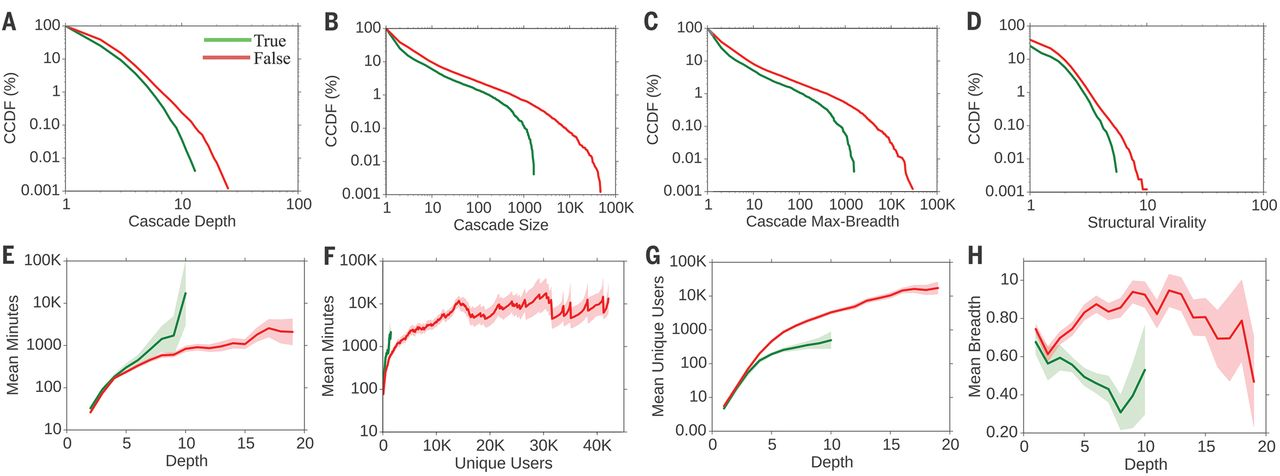
\includegraphics{figures/vosoughi.jpeg}

}

\caption{\citet{vosoughi2018}}

\end{figure}

ただし、インターネットを含めてマスメディアの影響を過大評価するべきではない。

\begin{itemize}
\tightlist
\item
  メディアの効果に関するサーベイとして \citet{inamasu2022} を参照。
\end{itemize}

\hypertarget{ux8cc7ux6e90ux3068ux3057ux3066ux306eux30c7ux30fcux30bf}{%
\section{資源としてのデータ}\label{ux8cc7ux6e90ux3068ux3057ux3066ux306eux30c7ux30fcux30bf}}

機械学習が調理法だとすれば、データは食材と言える。

\(\leadsto\)近年の機械学習の発展(後述)により、データの価値が発見(21世紀の資源と呼ばれることも)

\begin{itemize}
\tightlist
\item
  データそれ自体に価値があるわけではない。

  \begin{itemize}
  \tightlist
  \item
    適切な調理法(と下ごしらえ)がなければ宝の持ち腐れ。
  \end{itemize}
\end{itemize}

機械学習において、データの量が多いことは性能の向上に繋がる\href{https://deeplearning.hatenablog.com/entry/scaling_law}{スケーリング則}が発見されている。

\begin{figure}[htpb]

{\centering \includegraphics{big_data_files/mediabag/e047e8f1cde575800c5e.png}

}

\caption{\citet{kaplan2020}}

\end{figure}

\(\leadsto\)資源としてデータは足りるのか?

質の良いテキストデータは近いうちに\href{https://www.technologyreview.jp/s/291329/we-could-run-out-of-data-to-train-ai-language-programs/}{枯渇する可能性}が指摘されている。

\begin{itemize}
\tightlist
\item
  非デジタル情報のデジタル化?
\item
  ネットユーザーの拡大?
\item
  AI利用者の入力データの利用?
\end{itemize}


  \bibliography{references.bib}


\end{document}
